% ============================================================================
%  Hospital Management System — Project Report (v2)
%  Structure modelled on the "Travallae" reference report (KU, DoCSE).
%
%  Compiles with pdfLaTeX (Overleaf: press Recompile).
%  Diagrams are drawn in TikZ; screenshots live in pica/.
%  TODO before submitting: confirm items marked  % <-- VERIFY
% ============================================================================
\documentclass[12pt,a4paper]{report}

\usepackage[utf8]{inputenc}
\usepackage[T1]{fontenc}
\usepackage{lmodern}
\usepackage[margin=1in]{geometry}
\usepackage{graphicx}
\usepackage{setspace}
\usepackage{enumitem}
\usepackage{booktabs}
\usepackage{array}
\usepackage{xcolor}
\usepackage{tikz}
\usepackage{caption}
\usepackage[hidelinks]{hyperref}

\usetikzlibrary{shapes.geometric, arrows.meta, positioning, fit, calc}
\onehalfspacing

% ---- Real screenshot figure: \rfig{file}{caption}{label} -------------------
\newcommand{\rfig}[3]{%
  \begin{figure}[htbp]
  \centering
  \fbox{\includegraphics[width=0.86\textwidth]{#1}}
  \caption{#2}\label{#3}
  \end{figure}}

% ---- Flowchart / diagram node styles --------------------------------------
\tikzset{
  startstop/.style={rectangle, rounded corners, draw=black, fill=green!12, minimum width=2.7cm, minimum height=0.8cm, align=center, font=\small},
  process/.style={rectangle, draw=black, fill=blue!8, minimum width=3.2cm, minimum height=0.8cm, align=center, font=\small},
  decision/.style={diamond, aspect=2, draw=black, fill=orange!15, minimum width=2.6cm, align=center, inner sep=1pt, font=\small},
  io/.style={trapezium, trapezium left angle=70, trapezium right angle=110, draw=black, fill=yellow!15, minimum width=2.6cm, minimum height=0.7cm, align=center, font=\small},
  ent/.style={rectangle, rounded corners, draw=black, fill=blue!6, minimum width=2.4cm, minimum height=0.7cm, align=center, font=\small},
  arrow/.style={-{Stealth[length=2mm]}, thick},
}

\begin{document}

% ===========================================================================
% TITLE PAGE
% ===========================================================================
\begin{titlepage}
\centering

\includegraphics[width=2.8cm]{pica/logo.png}\par
\vspace{12pt}
{\Large\bfseries Kathmandu University\par}
\vspace{2pt}
{\large Department of Computer Science and Engineering\par}
{\large Dhulikhel, Kavre\par}
\vspace{1.8cm}
{\large A Project Report\par}
\vspace{4pt}
{\large on\par}
\vspace{10pt}
{\LARGE\bfseries ``Hospital Management System''\par}
\vspace{10pt}
{\large [Code No.: COMP 207]\par}                       % <-- VERIFY course code
\vspace{6pt}
{\normalsize (For partial fulfillment of Year II / Semester II in Computer Science)\par}
\vspace{1.6cm}
{\large\bfseries Submitted by\par}
\vspace{6pt}
{\normalsize
Aayush Aacharya (Roll no. 1)\\
Aayush Adhikari (Roll no. 2)\\
Aarjan Adhikari (Roll no. 3)\\
Krish Ghimire (Roll no. 24)\\ }                          % <-- VERIFY names / rolls
\vspace{1.4cm}
{\large\bfseries Submitted to\par}
\vspace{4pt}
{\normalsize Mr. Suman Shrestha\\                        % <-- VERIFY
Department of Computer Science and Engineering\par}
\vspace{1.4cm}
{\normalsize \today\par}                                 % <-- VERIFY submission date
\end{titlepage}

% ===========================================================================
% BONA FIDE CERTIFICATE
% ===========================================================================
\pagenumbering{roman}
\thispagestyle{plain}
\vspace*{\fill}
\begin{center}
{\Large\bfseries Bona fide Certificate}\\[1.1cm]
This project work on\\[4pt]
{\bfseries ``Hospital Management System''}\\[4pt]
is the bona fide work of\\[6pt]
\emph{Aayush Aacharya (Roll no. 1), Aayush Adhikari (Roll no. 2),\\
Aarjan Adhikari (Roll no. 3), Krish Ghimire (Roll no. 24)}\\[6pt]
who carried out the project work under my supervision.
\end{center}
\vspace{2.2cm}
\noindent
Project Supervisor\\[2pt]
\rule{6cm}{0.4pt}\\
Dr. Rabindra Bista\\                                     % <-- VERIFY supervisor
Department of Computer Science and Engineering
\vspace*{\fill}
\newpage

% ===========================================================================
% ACKNOWLEDGEMENTS
% ===========================================================================
\chapter*{Acknowledgements}
\addcontentsline{toc}{chapter}{Acknowledgements}
To everyone who contributed to the success of our project, we extend our heartfelt
appreciation. We are thankful for the collective efforts and support from all those
who contributed, directly or indirectly, to the successful completion of our project.
Their encouragement has been invaluable, and we truly appreciate the collaborative
spirit that made this endeavour possible.

A sincere gratitude goes to Dr. Rabindra Bista, our project supervisor. His
unwavering support, guidance, and constructive feedback have been instrumental in
steering our project towards excellence.

A special thanks to the Department of Computer Science and Engineering (DoCSE) for
providing an enriching academic environment and the necessary resources that played
a crucial role in the accomplishment of our team project.

% ===========================================================================
% ABSTRACT
% ===========================================================================
\chapter*{Abstract}
\addcontentsline{toc}{chapter}{Abstract}
Hospital operations often become inefficient, and patient care is affected, because
many hospitals rely on manual processes or disconnected management tools. This
project developed a full-stack \textbf{Hospital Management System (HMS)} that unifies
core clinical and administrative operations on a single digital platform. The system
was implemented using a layered client--server architecture to improve scalability,
maintainability, and security. The backend was developed using Node.js, Express, and
the Sequelize ORM over a MySQL relational database, while a responsive web interface
was built with React and Tailwind CSS to serve five distinct roles---patient, doctor,
pharmacist, lab assistant, and administrator. Secure authentication was implemented
using JSON Web Tokens (JWT) with refresh-token rotation, together with role-based
access control, password reset, and email verification. The completed system provides
features such as appointment scheduling with doctor availability, prescriptions,
laboratory-test workflows, referrals, billing and invoicing, a location-aware pharmacy
inventory, and multi-channel notifications delivered in-app and by email. In
conclusion, the HMS successfully delivers a secure, scalable, and user-friendly
hospital-management solution, and future enhancements are recommended, including
database migrations, an inpatient/ward module, and predictive analytics.

\vspace{0.4cm}
\noindent\textbf{Keywords:} Hospital Management System, React, Node.js, Express,
MySQL, Sequelize, JWT, Role-Based Access Control, RESTful API.

% ===========================================================================
% CONTENTS / FIGURES
% ===========================================================================
\tableofcontents
\listoffigures

% ===========================================================================
% ABBREVIATIONS
% ===========================================================================
\chapter*{Abbreviations}
\addcontentsline{toc}{chapter}{Abbreviations}
\begin{tabular}{@{}p{3cm}p{11cm}@{}}
HMS     & Hospital Management System. \\
REST    & Representational State Transfer. \\
API     & Application Programming Interface. \\
JWT     & JSON Web Token. \\
ORM     & Object--Relational Mapping. \\
RBAC    & Role-Based Access Control. \\
SPA     & Single Page Application. \\
CRUD    & Create, Read, Update, Delete. \\
SMTP    & Simple Mail Transfer Protocol. \\
VS Code & Visual Studio Code. \\
\end{tabular}

% ===========================================================================
\clearpage
\pagenumbering{arabic}

% ===========================================================================
% CHAPTER 1 — INTRODUCTION
% ===========================================================================
\chapter{Introduction}
The Hospital Management System (HMS) is a role-based web platform developed to
connect the different people involved in patient care---patients, doctors, pharmacists,
lab assistants, and administrators---through a single digital system. It provides a
web interface where patients can register, book appointments, view prescriptions and
lab results, and settle bills, while hospital staff manage schedules, clinical records,
pharmacy stock, and billing. The system focuses on making everyday hospital tasks
simple and reliable while keeping medical data secure. By using modern technologies,
it supports consistent records and timely notifications, helping to reduce the common
problems found in manual and disconnected hospital systems.

\section{Background}
The rapid growth of digital technology has changed how hospitals manage information.
Patients increasingly expect to book appointments and view records online, while
hospitals adopt web-based systems to manage scheduling, prescriptions, laboratory
work, and billing, with modern solutions focusing on user-friendly design, reliable
records, and secure access.

However, many existing systems have limitations. Some focus mainly on record-keeping
while offering little role separation, and others are too complex or costly for small
and medium-sized institutions. In many cases, hospitals rely on separate tools for
appointments, pharmacy, and billing, which increases complexity and reduces
efficiency. Sensitive medical data also demands strong authentication and access
control that older systems often lack.

These issues highlight the need for a more balanced and integrated system. The HMS
addresses this by combining appointment scheduling, clinical records, pharmacy
inventory, billing, and notifications within one secure, role-based platform,
improving interaction between patients and staff and increasing overall efficiency.

\section{Objectives}
The main objectives achieved during the development of the HMS were:
\begin{itemize}[leftmargin=1.4em]
  \item Developed a web-based platform that enabled patients to register, book, and
        manage appointments efficiently.
  \item Created role-specific dashboards that allowed doctors, pharmacists, lab
        assistants, and administrators to manage their respective operations.
  \item Implemented core clinical and administrative workflows---prescriptions,
        laboratory tests, referrals, billing, and a location-aware pharmacy inventory.
  \item Ensured secure user authentication and role-based access control using JWT
        with refresh-token rotation, password reset, and email verification.
  \item Provided multi-channel notifications (in-app and email) so users stay
        informed without needing to log in.
\end{itemize}

\section{Motivation and Significance}
The motivation behind this project was to gain hands-on experience building a
real-world, full-stack web application while addressing the practical limitations of
manual and fragmented hospital systems. Most modern institutions depend on digital
systems to manage appointments, records, and billing, and recent solutions emphasise
simple interfaces, reliable data, and secure access using modern technologies.

The significance of the HMS lies in its ability to improve operational efficiency,
reduce manual errors, and offer secure, role-based access to clinical and
administrative information. By combining scheduling, prescriptions, laboratory
workflows, pharmacy inventory, billing, and notifications in a single platform, the
system makes hospital operations more efficient and easier to use for both patients
and staff, while providing a scalable foundation for future enhancement.

% ===========================================================================
% CHAPTER 2 — RELATED WORKS
% ===========================================================================
\chapter{Related Works}
Hospital information systems have evolved significantly with the adoption of digital
platforms that manage patient records, scheduling, pharmacy, and billing. Modern
systems provide electronic health records, appointment management, secure access, and
reporting. While these platforms have transformed healthcare delivery, many existing
solutions either focus on large enterprise deployments or require complex configuration
unsuitable for small institutions. This chapter reviews existing hospital-management
platforms related to the proposed HMS and identifies the gaps it aims to address.

\section{Review of Existing Works}

\subsection*{OpenMRS}
OpenMRS is a widely used open-source medical-record platform designed to support
healthcare delivery, particularly in resource-constrained settings. OpenMRS (2026)
\begin{itemize}[leftmargin=1.4em, itemsep=1pt]
  \item \textbf{Technologies / Methodology:} Java-based web platform with a
        configurable data model for patients, encounters, and observations, extended
        through a modular architecture.
  \item \textbf{Strengths:} Centralised patient record, role-based access, active
        global community, and high configurability.
  \item \textbf{Limitations:} Requires a dedicated server environment and technical
        expertise to install, configure, and maintain, which is a barrier for small
        institutions without dedicated IT staff.
\end{itemize}
While OpenMRS provides a comprehensive medical-record platform, the proposed HMS
focuses on a simpler, integrated solution that combines appointments, pharmacy, and
billing in one role-based system tailored for small and medium-sized hospitals.

\subsection*{OpenEMR}
OpenEMR is a mature open-source electronic health record and practice-management
system used by clinics and hospitals worldwide. OpenEMR (2026)
\begin{itemize}[leftmargin=1.4em, itemsep=1pt]
  \item \textbf{Technologies / Methodology:} PHP and MySQL web application supporting
        scheduling, prescriptions, billing, and reporting.
  \item \textbf{Strengths:} Feature-rich, certified for clinical use, and supported
        by an established community.
  \item \textbf{Limitations:} Its breadth brings configuration complexity, and its
        older architecture is less suited to lightweight deployment or full-stack
        learning environments.
\end{itemize}
Compared to OpenEMR, the proposed HMS delivers the core functionalities required for
efficient hospital management using a modern, modular full-stack architecture that is
simpler to deploy and understand.

\subsection*{HospitalRun}
HospitalRun is an open-source hospital information system aimed at small and rural
hospitals, with an emphasis on offline-first operation. HospitalRun (2026)
\begin{itemize}[leftmargin=1.4em, itemsep=1pt]
  \item \textbf{Technologies / Methodology:} JavaScript-based platform covering
        patient records, scheduling, billing, and inventory, designed to work in
        low-connectivity environments.
  \item \textbf{Strengths:} Usability focus and reliable operation where connectivity
        is limited.
  \item \textbf{Limitations:} Feature set and active maintenance vary across releases,
        and role separation is limited compared with enterprise systems.
\end{itemize}
Unlike HospitalRun, the proposed HMS provides fine-grained role-based access across
five distinct roles and integrates pharmacy inventory, billing, and multi-channel
notifications within a single, actively structured codebase.

% ===========================================================================
% CHAPTER 3 — DESIGN AND IMPLEMENTATION
% ===========================================================================
\chapter{Design and Implementation}
The Hospital Management System is a role-based web platform developed to connect
patients and hospital staff through a single digital system. It provides role-specific
dashboards that allow patients to book appointments and view records, and staff to
manage schedules, prescriptions, laboratory work, pharmacy stock, and billing.

\section{System Overview}
The HMS addresses the need for a simple, integrated hospital platform by bringing
appointments, clinical records, pharmacy, billing, and notifications together in one
secure, role-based system. Each role interacts only with the features appropriate to
it, and all data flows through a single backend over a well-defined RESTful API.

\subsection{Major Components}
\begin{itemize}[leftmargin=1.4em]
  \item \textbf{Frontend Development:} The web interface is developed using React.js
        with the Vite build tool. Tailwind CSS is used for styling, React Router for
        client-side navigation, and Axios as the API client for communicating with the
        backend.
  \item \textbf{Backend Development:} Node.js with the Express.js framework is used for
        server-side development. The backend follows a REST API architecture for
        client--server communication, with MySQL as the relational database accessed
        through the Sequelize Object--Relational Mapping (ORM) library. JSON Web Tokens
        secure the API, and Nodemailer provides outbound email.
  \item \textbf{Development Tools:} Visual Studio Code (VS Code) is used as the primary
        code editor. Git and GitHub are used for version control and source-code
        management, Nodemon for automatic server reloading during development, and
        ESLint for code quality.
\end{itemize}

\subsection{Component Interaction}
\begin{itemize}[leftmargin=1.4em]
  \item Patients and staff interact with the React web application to perform
        role-specific actions such as booking appointments, issuing prescriptions,
        processing lab tests, managing pharmacy stock, and settling invoices.
  \item The frontend communicates with the backend through RESTful APIs over HTTP,
        under the common base path \texttt{/api/v1/hms}. The backend processes
        requests, performs business logic, and returns JSON responses.
  \item The backend authenticates users using JWT-based authentication and authorises
        access based on user roles before performing CRUD operations on the MySQL
        database through Sequelize.
  \item Access tokens are short-lived and refreshed through rotating refresh tokens
        stored in HTTP-only cookies, which can be revoked to end all sessions.
  \item External services, such as the email (SMTP) and SMS providers, are invoked by
        the backend to send appointment, prescription, billing, and account
        notifications to users.
\end{itemize}

\section{System Requirement Specifications}

\subsection{Software Requirements}
\paragraph{Frontend Development}
\begin{itemize}[leftmargin=1.4em, itemsep=0pt]
  \item \textbf{Programming Language:} JavaScript (ES2022)
  \item \textbf{Frameworks / Libraries:} React.js, Vite
  \item \textbf{Styling:} Tailwind CSS
  \item \textbf{API Client:} Axios
\end{itemize}
\paragraph{Backend Development}
\begin{itemize}[leftmargin=1.4em, itemsep=0pt]
  \item \textbf{Programming Language:} JavaScript (Node.js)
  \item \textbf{Framework:} Express.js
  \item \textbf{API Architecture:} Representational State Transfer (REST) API
  \item \textbf{Database:} MySQL with the Sequelize ORM
  \item \textbf{Authentication / Email:} JSON Web Tokens, bcrypt, Nodemailer
\end{itemize}
\paragraph{Development Tools}
\begin{itemize}[leftmargin=1.4em, itemsep=0pt]
  \item \textbf{Code Editor:} Visual Studio Code (VS Code)
  \item \textbf{Version Control:} Git, GitHub
  \item \textbf{Runtime Tooling:} Nodemon, ESLint
  \item \textbf{Operating System:} Windows
\end{itemize}

\subsection{Functional Requirements}
\begin{itemize}[leftmargin=1.4em]
  \item Users shall be able to register, log in, and manage their accounts securely,
        with password reset and email verification.
  \item Patients shall be able to book, view, and cancel appointments based on doctor
        availability.
  \item Doctors shall be able to issue prescriptions, order laboratory tests, and refer
        patients to other doctors.
  \item Lab assistants shall be able to process test requests and record results, which
        patients can then view.
  \item Administrators shall be able to manage staff accounts, rooms, and billing.
  \item Pharmacists shall be able to manage a location-aware medicine inventory with
        stock levels and reorder thresholds.
  \item The system shall create in-app notifications and deliver them by email.
\end{itemize}

\subsection{Non-Functional Requirements}
\begin{itemize}[leftmargin=1.4em]
  \item The system shall provide a responsive and user-friendly interface across major
        web browsers.
  \item The system shall support multiple concurrent users while maintaining consistent
        performance.
  \item The system shall ensure secure authentication and protect medical data from
        unauthorised access.
  \item The system shall be scalable and maintainable to accommodate future features.
\end{itemize}

\section{System Design}

\subsection{Architectural Design}
The HMS follows a layered client--server architecture. The presentation layer (React
SPA) renders role-specific dashboards and calls the backend over REST; the application
layer (Express) enforces authentication, authorisation, and business logic through
controllers, middleware, and services; and the data layer (MySQL via Sequelize) stores
all persistent records with enforced relationships. Figure~\ref{fig:arch} shows the
overall architecture.

\begin{figure}[htbp]
\centering
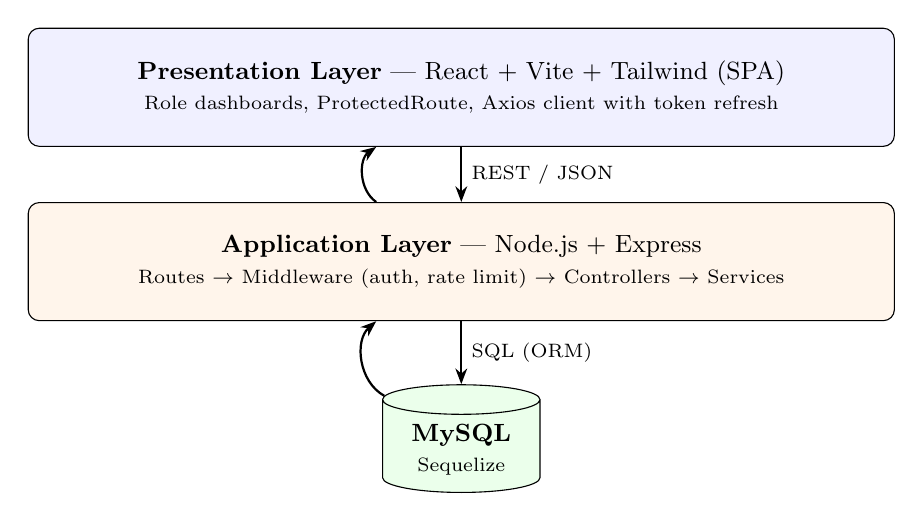
\begin{tikzpicture}[font=\small, node distance=0.9cm,
  layer/.style={draw, rounded corners, minimum width=11cm, minimum height=1.5cm, align=center},
  db/.style={draw, cylinder, shape border rotate=90, aspect=0.25, minimum width=2cm, minimum height=1.3cm, align=center, fill=green!8}]
\node[layer, fill=blue!6] (pres) {\textbf{Presentation Layer} — React + Vite + Tailwind (SPA)\\
  \scriptsize Role dashboards, ProtectedRoute, Axios client with token refresh};
\node[layer, fill=orange!8, below=0.7cm of pres] (app) {\textbf{Application Layer} — Node.js + Express\\
  \scriptsize Routes $\rightarrow$ Middleware (auth, rate limit) $\rightarrow$ Controllers $\rightarrow$ Services};
\node[db, below=0.8cm of app] (data) {\textbf{MySQL}\\\scriptsize Sequelize};
\draw[arrow] (pres) -- node[right]{\scriptsize REST / JSON} (app);
\draw[arrow] (app) -- node[right]{\scriptsize SQL (ORM)} (data);
\draw[arrow] (data) to[bend left=55] (app);
\draw[arrow] (app) to[bend left=55] (pres);
\end{tikzpicture}
\caption{System architecture}
\label{fig:arch}
\end{figure}

\subsection{Database Design}
The HMS uses MySQL as its primary database to store application data. The schema is
normalised into related tables for the key entities, including \textbf{Users},
\textbf{Patients}, \textbf{Staff Profiles}, \textbf{Appointments},
\textbf{Prescriptions}, \textbf{Lab Tests}, \textbf{Referrals}, \textbf{Invoices},
\textbf{Medicines}, and \textbf{Notifications}. Relationships between tables are
enforced using foreign keys with cascade rules, allowing efficient and consistent data
retrieval. This schema provides the integrity and scalability required to support
scheduling, clinical records, billing, and pharmacy management. Figure~\ref{fig:er}
shows the entity--relationship overview.

\begin{figure}[htbp]
\centering
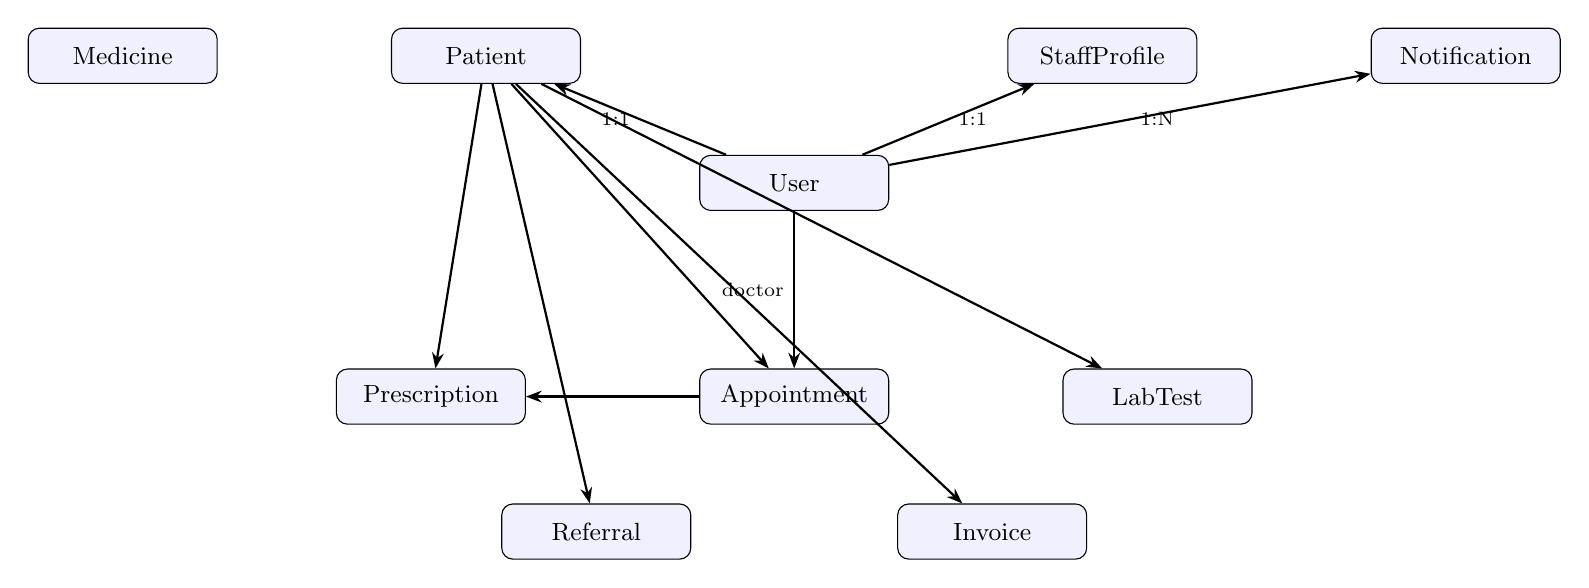
\begin{tikzpicture}[node distance=0.8cm and 1.4cm]
\node[ent] (user) {User};
\node[ent, above left=0.9cm and 1.5cm of user] (patient) {Patient};
\node[ent, above right=0.9cm and 1.5cm of user] (staff) {StaffProfile};
\node[ent, below=2.0cm of user] (appt) {Appointment};
\node[ent, left=2.2cm of appt] (presc) {Prescription};
\node[ent, right=2.2cm of appt] (lab) {LabTest};
\node[ent, below left=1.0cm and 0.1cm of appt] (refer) {Referral};
\node[ent, below right=1.0cm and 0.1cm of appt] (invoice) {Invoice};
\node[ent, right=2.2cm of staff] (notif) {Notification};
\node[ent, left=2.2cm of patient] (med) {Medicine};
\draw[arrow] (user) -- node[left,font=\scriptsize]{1:1} (patient);
\draw[arrow] (user) -- node[right,font=\scriptsize]{1:1} (staff);
\draw[arrow] (user) -- node[right,font=\scriptsize]{1:N} (notif);
\draw[arrow] (patient) -- (appt);
\draw[arrow] (user) -- node[left,font=\scriptsize]{doctor} (appt);
\draw[arrow] (patient) -- (presc);
\draw[arrow] (patient) -- (lab);
\draw[arrow] (patient) -- (refer);
\draw[arrow] (patient) -- (invoice);
\draw[arrow] (appt) -- (presc);
\end{tikzpicture}
\caption{ER diagram (principal entities and relationships)}
\label{fig:er}
\end{figure}

\section{Implementation Details}
This section describes how the proposed architecture was implemented. The system was
developed using a layered client--server architecture consisting of a React web
application and an Express backend, integrated through RESTful APIs to provide a
seamless hospital-management experience.

\subsection{Frontend Implementation}
The frontend is a Single Page Application developed using React.js, Vite, and Tailwind
CSS. It provides role-specific dashboards for patients, doctors, pharmacists, lab
assistants, and administrators. A \texttt{ProtectedRoute} component restricts each
dashboard to its allowed roles, authentication state is held in a React context, and
Axios attaches the JWT access token to every request while transparently refreshing it
on expiry. Toast notifications provide user feedback.

\subsection{Backend Implementation}
The backend was developed using Node.js, Express.js, and the Sequelize ORM in a modular
structure with separate routes, controllers, middleware, and services. Controllers
handle authentication, appointments, availability, prescriptions, lab tests, referrals,
invoices, notifications, medicines, and staff. Middleware enforces JWT authentication,
role-based authorisation, and rate limiting on sensitive endpoints, while MySQL stores
all persistent data. Password hashes use bcrypt, and reset/verification tokens are
stored only as SHA-256 hashes.

\subsection{Integration of Components}
The frontend communicates with the backend through RESTful APIs over HTTP. The backend
interacts with MySQL through Sequelize for persistent storage and enforces referential
integrity with foreign-key relationships. External services, including the email (SMTP)
and SMS providers, are integrated with the backend to send notifications; when these are
not configured, the system falls back to console logging so all flows remain runnable in
development. This modular implementation keeps the system scalable, maintainable, and
easy to extend.

\section{Flowcharts}
This section presents the flowcharts illustrating the workflow and system logic of the
HMS. They describe the sequence of operations for user registration, authentication,
appointment booking, and role-based access, showing how users and the backend interact
to complete operations within the system.

\begin{figure}[htbp]
\centering
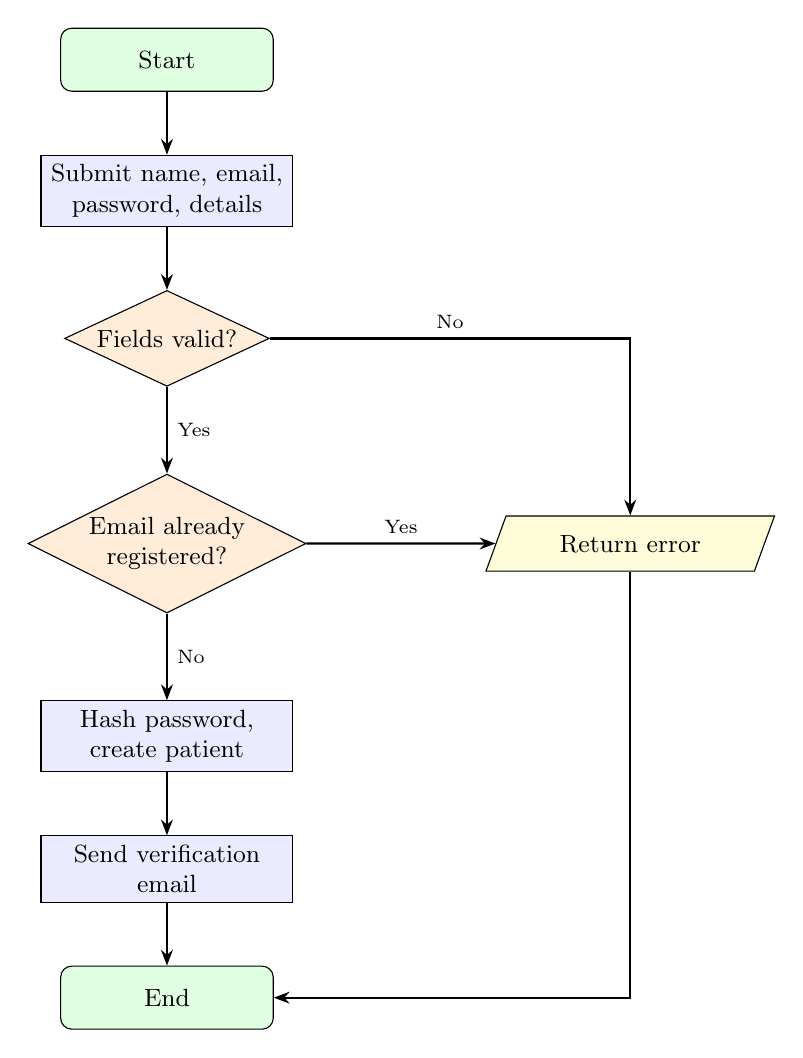
\begin{tikzpicture}[node distance=0.8cm and 1.2cm]
\node[startstop] (s){Start};
\node[process, below=of s] (form){Submit name, email,\\password, details};
\node[decision, below=of form] (valid){Fields valid?};
\node[decision, below=1.1cm of valid] (exists){Email already\\registered?};
\node[process, below=1.1cm of exists] (hash){Hash password,\\create patient};
\node[process, below=of hash] (mail){Send verification\\email};
\node[startstop, below=of mail] (e){End};
\node[io, right=2.4cm of exists] (err){Return error};
\draw[arrow](s)--(form); \draw[arrow](form)--(valid);
\draw[arrow](valid)-- node[right,font=\scriptsize]{Yes}(exists);
\draw[arrow](exists)-- node[right,font=\scriptsize]{No}(hash);
\draw[arrow](hash)--(mail); \draw[arrow](mail)--(e);
\draw[arrow](valid)-| node[near start,above,font=\scriptsize]{No}(err);
\draw[arrow](exists)-- node[above,font=\scriptsize]{Yes}(err);
\draw[arrow](err)|-(e);
\end{tikzpicture}
\caption{Registration flowchart}
\label{fig:flow-reg}
\end{figure}

\begin{figure}[htbp]
\centering
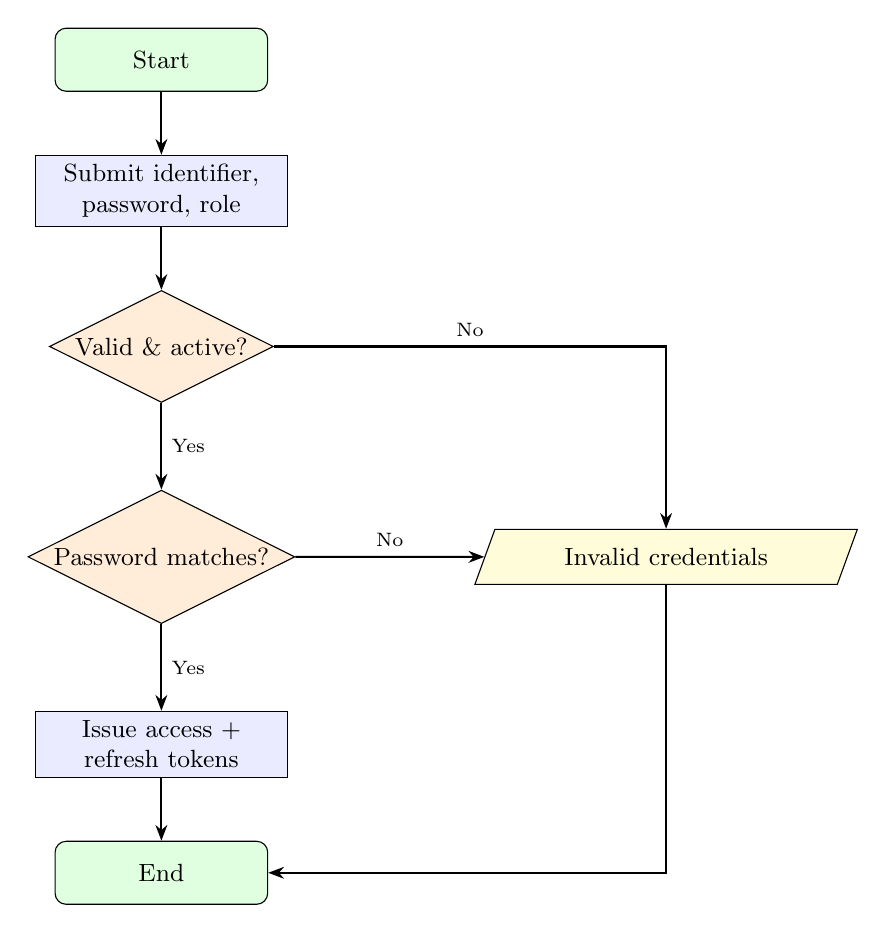
\begin{tikzpicture}[node distance=0.8cm and 1.2cm]
\node[startstop] (s){Start};
\node[process, below=of s] (sub){Submit identifier,\\password, role};
\node[decision, below=of sub] (val){Valid \& active?};
\node[decision, below=1.1cm of val] (pw){Password matches?};
\node[process, below=1.1cm of pw] (tok){Issue access +\\refresh tokens};
\node[startstop, below=of tok] (e){End};
\node[io, right=2.4cm of pw] (err){Invalid credentials};
\draw[arrow](s)--(sub); \draw[arrow](sub)--(val);
\draw[arrow](val)-- node[right,font=\scriptsize]{Yes}(pw);
\draw[arrow](pw)-- node[right,font=\scriptsize]{Yes}(tok);
\draw[arrow](tok)--(e);
\draw[arrow](val)-| node[near start,above,font=\scriptsize]{No}(err);
\draw[arrow](pw)-- node[above,font=\scriptsize]{No}(err);
\draw[arrow](err)|-(e);
\end{tikzpicture}
\caption{Login flowchart}
\label{fig:flow-login}
\end{figure}

\begin{figure}[htbp]
\centering
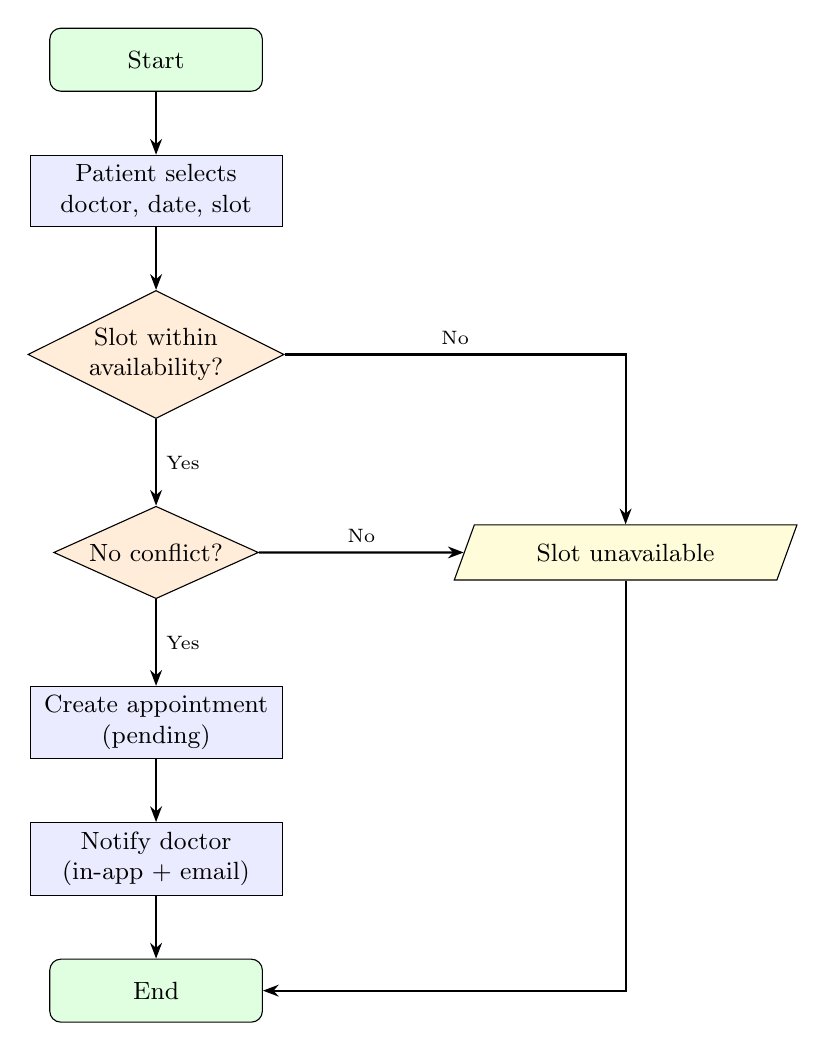
\begin{tikzpicture}[node distance=0.8cm and 1.3cm]
\node[startstop] (s){Start};
\node[process, below=of s] (pick){Patient selects\\doctor, date, slot};
\node[decision, below=of pick] (avail){Slot within\\availability?};
\node[decision, below=1.1cm of avail] (free){No conflict?};
\node[process, below=1.1cm of free] (create){Create appointment\\(pending)};
\node[process, below=of create] (notify){Notify doctor\\(in-app + email)};
\node[startstop, below=of notify] (e){End};
\node[io, right=2.6cm of free] (err){Slot unavailable};
\draw[arrow](s)--(pick); \draw[arrow](pick)--(avail);
\draw[arrow](avail)-- node[right,font=\scriptsize]{Yes}(free);
\draw[arrow](free)-- node[right,font=\scriptsize]{Yes}(create);
\draw[arrow](create)--(notify); \draw[arrow](notify)--(e);
\draw[arrow](avail)-| node[near start,above,font=\scriptsize]{No}(err);
\draw[arrow](free)-- node[above,font=\scriptsize]{No}(err);
\draw[arrow](err)|-(e);
\end{tikzpicture}
\caption{Appointment booking flowchart}
\label{fig:flow-appt}
\end{figure}

\begin{figure}[htbp]
\centering
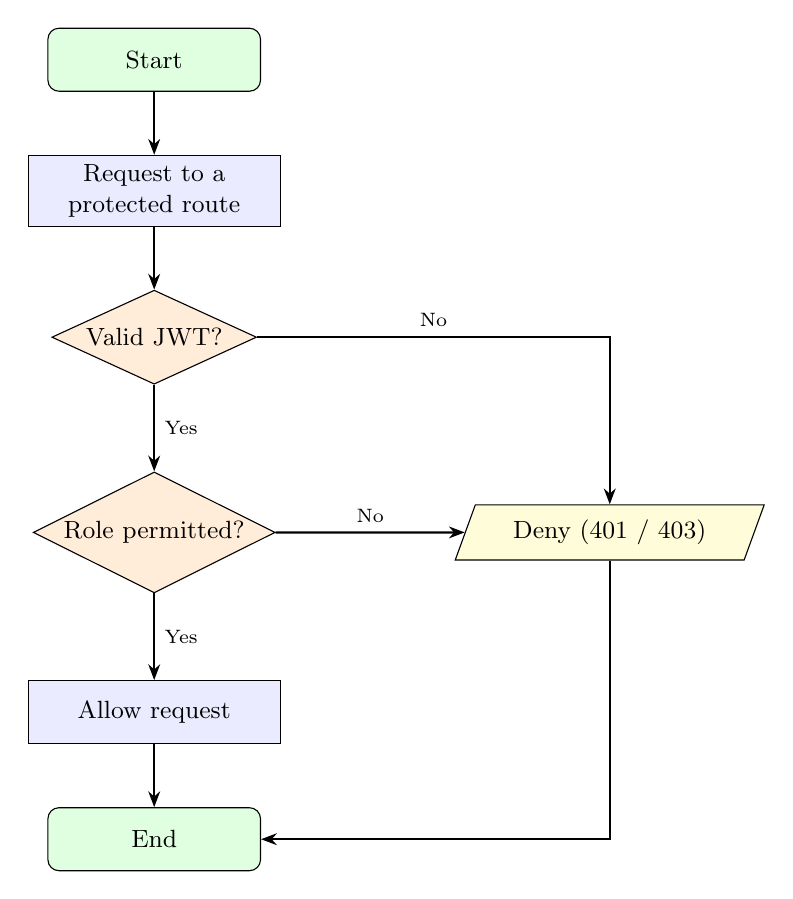
\begin{tikzpicture}[node distance=0.8cm and 1.2cm]
\node[startstop] (s){Start};
\node[process, below=of s] (req){Request to a\\protected route};
\node[decision, below=of req] (jwt){Valid JWT?};
\node[decision, below=1.1cm of jwt] (role){Role permitted?};
\node[process, below=1.1cm of role] (ok){Allow request};
\node[startstop, below=of ok] (e){End};
\node[io, right=2.4cm of role] (deny){Deny (401 / 403)};
\draw[arrow](s)--(req); \draw[arrow](req)--(jwt);
\draw[arrow](jwt)-- node[right,font=\scriptsize]{Yes}(role);
\draw[arrow](role)-- node[right,font=\scriptsize]{Yes}(ok);
\draw[arrow](ok)--(e);
\draw[arrow](jwt)-| node[near start,above,font=\scriptsize]{No}(deny);
\draw[arrow](role)-- node[above,font=\scriptsize]{No}(deny);
\draw[arrow](deny)|-(e);
\end{tikzpicture}
\caption{Role-based access control flowchart}
\label{fig:flow-rbac}
\end{figure}

% ===========================================================================
% CHAPTER 4 — RESULTS AND DISCUSSION
% ===========================================================================
\chapter{Results and Discussion}

\section{Implemented Features}
The Hospital Management System successfully implemented several core functionalities:
\begin{itemize}[leftmargin=1.4em]
  \item \textbf{User Authentication:} Users register and log in using JWT-based
        authentication with refresh-token rotation, together with password reset and
        email verification, ensuring protected access to authorised resources.
  \item \textbf{Role-Based Dashboards:} Each of the five roles (patient, doctor,
        pharmacist, lab assistant, administrator) has a distinct dashboard exposing
        only its permitted features.
  \item \textbf{Appointment Management:} Patients book appointments against a doctor's
        declared availability with conflict checking, and appointments follow a
        pending/confirmed/cancelled/completed workflow.
  \item \textbf{Clinical Records:} Doctors issue prescriptions, order laboratory tests,
        and refer patients; lab assistants process test requests and record results.
  \item \textbf{Billing and Pharmacy:} Administrators issue invoices and record
        payments, while pharmacists manage a location-aware medicine catalogue with
        stock levels, reorder thresholds, and expiry.
  \item \textbf{Notifications:} In-app notifications are created for key events and
        mirrored to the user's email, keeping users informed without logging in.
\end{itemize}
Figures~\ref{fig:login}--\ref{fig:pharm} in Appendix~A show the running system.

\section{Results and Performance Analysis}
The implemented system was tested to evaluate its functionality, performance, and
reliability. Testing confirmed that the core features operated correctly:
\begin{itemize}[leftmargin=1.4em]
  \item \textbf{Authentication:} JWT-based authentication allowed secure registration,
        login, and access to protected resources while preventing unauthorised access;
        password reset revoked existing sessions correctly.
  \item \textbf{Appointment and Clinical Records:} Appointments, prescriptions, lab
        tests, and referrals were created and updated successfully, with records stored
        and retrieved accurately from MySQL.
  \item \textbf{Billing and Pharmacy:} Invoices and payments were recorded with correct
        status transitions, and the medicine catalogue displayed accurate stock and
        location data.
  \item \textbf{Database Performance:} MySQL handled CRUD operations for users,
        appointments, and invoices with quick response times under normal load.
  \item \textbf{System Stability:} The backend started, connected to the database,
        synchronised all models, and served requests without major errors; the frontend
        built and ran without runtime errors.
\end{itemize}

\section{Comparison with Objectives or Existing Systems}
The implemented system successfully achieves its primary objectives by providing an
integrated platform for hospital management through a role-based web application.
During analysis and design, existing systems such as OpenMRS, OpenEMR, and HospitalRun
were studied to understand their features and workflows. Unlike these platforms---which
offer broad enterprise features but require significant configuration---the proposed
system focuses on the core functionalities required for efficient hospital management:
secure authentication, appointments, prescriptions, laboratory workflows, referrals,
billing, and pharmacy inventory, within a simple and maintainable full-stack codebase.

Some deviations from the original plan:
\begin{itemize}[leftmargin=1.4em]
  \item \textbf{Managed migrations:} the schema is auto-synchronised in development
        rather than versioned through migrations.
  \item \textbf{Transactions:} some multi-step flows (such as recording payments) are
        not yet fully transactional.
  \item \textbf{SMS delivery:} notifications are delivered in-app and by email; SMS is
        supported but disabled unless a provider is configured.
  \item \textbf{Inpatient module:} ward and bed management were considered but reserved
        for future development.
\end{itemize}

\section{Discussion}
The implementation demonstrates the effectiveness of modern web technologies in
building a unified hospital-management platform. By combining a React frontend, an
Express backend, and a MySQL database accessed through Sequelize, the system provides a
consistent and responsive experience. REST APIs enable clean communication between the
frontend and backend, while JWT-based authentication with refresh-token rotation ensures
secure, revocable access. The layered, modular architecture improves maintainability and
allows new features to be added with minimal changes. The normalised relational schema
efficiently manages relationships among patients, staff, appointments, and billing,
keeping the system scalable for future expansion such as an inpatient module, audit
logging, and analytics.

% ===========================================================================
% CHAPTER 5 — CONCLUSION AND FUTURE WORKS
% ===========================================================================
\chapter{Conclusion and Future Works}
The Hospital Management System was successfully designed and implemented using modern
web development technologies to provide a secure, role-based platform for patients and
hospital staff. The system adopts a layered client--server architecture, with React
powering the web application and Node.js with Express handling backend services. MySQL,
accessed through Sequelize, serves as the primary database, offering a reliable and
scalable solution for storing clinical and administrative records. Secure authentication
is achieved through JWT with refresh-token rotation, while communication between the
frontend and backend uses REST APIs. The implementation provides essential features such
as appointment scheduling, prescriptions, laboratory workflows, referrals, billing, and
pharmacy inventory, with notifications delivered in-app and by email. Overall, the
proposed system is efficient, reliable, scalable, and user-friendly, providing a solid
foundation for future enhancements.

\section{Limitations}
Although the proposed system implements the core functionalities required for hospital
management, it has several limitations that can be addressed in future versions.
\begin{itemize}[leftmargin=1.4em]
  \item The database schema is auto-synchronised in development rather than managed
        through versioned migrations.
  \item Some multi-step operations are not yet fully transactional.
  \item Real email and SMS delivery depend on external providers being configured;
        otherwise messages fall back to console logging.
  \item The system is web-only, with no dedicated mobile application.
  \item An automated test suite is not yet in place; verification is currently manual.
  \item Inpatient/ward management and audit logging are not yet implemented.
\end{itemize}

\section{Future Enhancements}
Several improvements can be incorporated into future versions:
\begin{itemize}[leftmargin=1.4em]
  \item Adopt versioned database migrations and wrap critical flows (payments, booking)
        in transactions.
  \item Add an automated test suite with continuous integration.
  \item Implement an inpatient/ward and bed-management module.
  \item Introduce audit logging of access to medical data to support privacy and
        compliance.
  \item Add automatic pharmacy stock deduction on dispensing and low-stock alerts.
  \item Develop a companion mobile application for patients.
  \item Expand analytics with dashboards tracking hospital usage and trends.
\end{itemize}

% ===========================================================================
% REFERENCES
% ===========================================================================
\begin{thebibliography}{9}
\addcontentsline{toc}{chapter}{References}
\bibitem{openmrs} OpenMRS (2026). \emph{OpenMRS.} \url{https://openmrs.org/}. Accessed: \today.
\bibitem{openemr} OpenEMR (2026). \emph{OpenEMR.} \url{https://www.open-emr.org/}. Accessed: \today.
\bibitem{hospitalrun} HospitalRun (2026). \emph{HospitalRun.} \url{https://hospitalrun.io/}. Accessed: \today.
\bibitem{react} React (2026). \emph{React documentation.} \url{https://react.dev/}. Accessed: \today.
\bibitem{node} Node.js (2026). \emph{Node.js documentation.} \url{https://nodejs.org/en/docs/}. Accessed: \today.
\bibitem{sequelize} Sequelize (2026). \emph{Sequelize ORM documentation.} \url{https://sequelize.org/}. Accessed: \today.
\bibitem{mysql} MySQL (2026). \emph{MySQL documentation.} \url{https://dev.mysql.com/doc/}. Accessed: \today.
\end{thebibliography}

% ===========================================================================
% APPENDIX A
% ===========================================================================
\appendix
\chapter{Additional Figures and Screenshots}
\rfig{pica/log.png}{Login}{fig:login}
\rfig{pica/forgotpw.png}{Forgot password}{fig:forgotpw}
\rfig{pica/patient.png}{Patient dashboard}{fig:patient}
\rfig{pica/doctor.png}{Doctor dashboard}{fig:doctor}
\rfig{pica/admin.png}{Admin dashboard}{fig:admin}
\rfig{pica/appointment.png}{Appointment booking and management}{fig:appointment}
\rfig{pica/lab.png}{Lab Assistant portal}{fig:lab}
\rfig{pica/pharm.png}{Pharmacist portal — medicine inventory}{fig:pharm}

\end{document}
